\section*{Агентные модели. Дискретное пространство}
\addcontentsline{toc}{section}{Агентные модели. Дискретное пространство}
\subsection*{<<Жизнь>> Конвея}
\addcontentsline{toc}{subsection}{<<Жизнь>> Конвея}

\textbf{Задание:}\\
Реализовать модель <<Game Of Life>>\\

\textbf{Решение:}\\
Сначала была создана популяция размером -- 2500 агентов, заданная в дискретном пространстве и имеющую тип соседства -- Мурово. (Рисунок \ref{fig:game_of_life1})
\begin{figure}[h]
	\centering 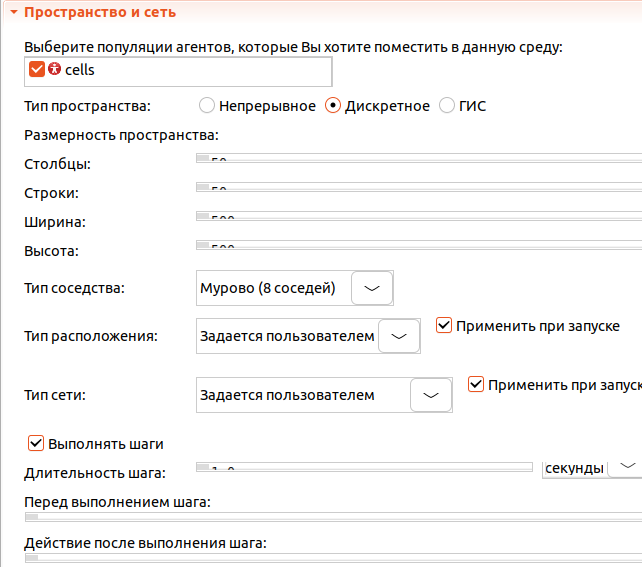
\includegraphics[scale=0.4]{game_of_life1}
	\caption{Настройка популяции агентов}
	\label{fig:game_of_life1}
\end{figure}

Цель данной модели заключается в том, что изначально каждой клетке присваивается состояние -- жива или мёртва. Далее это состояние изменяется, если рядом с живой клеткой находится меньше двух или больше трёх живых клеток, то она умирает. Мёртвая клетка, рядом с которой находится ровно три живые клетки, оживает.\\

\newpage

Для того чтобы реализовать данный алгоритм нужно перейти в популяцию агентов и задать действия перед выполнением шага и задать действие на каждом шаге. (Рисунок \ref{fig:game_of_life2})
\begin{figure}[h]
	\centering 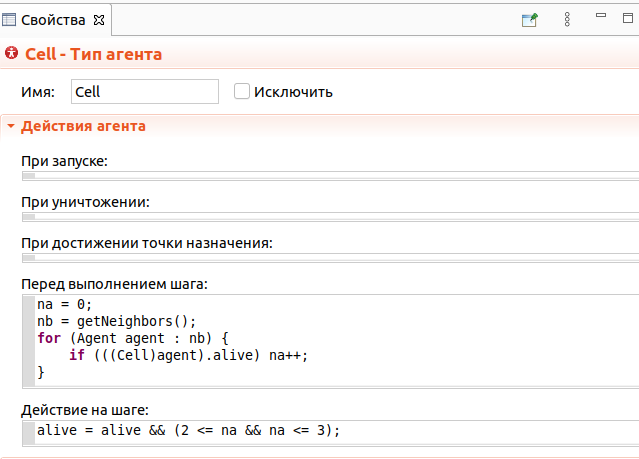
\includegraphics[scale=0.4]{game_of_life2}
	\caption{Реализация алгоритма Игры в жизнь}
	\label{fig:game_of_life2}
\end{figure}

В результате получается модель, в которой в соответствии с описанным алгоритмом меняются состояния клеток. Также можно поменять состояние клетки шёлкнув по ней. (Рисунок \ref{fig:game_of_life3})
\begin{figure}[h]
	\centering 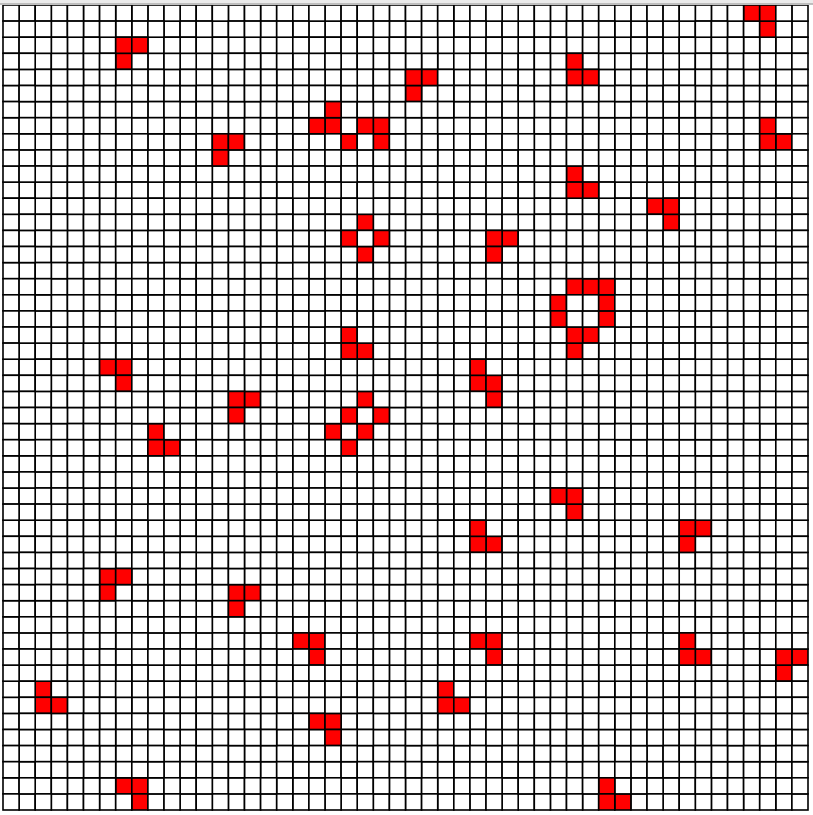
\includegraphics[scale=0.27]{game_of_life3}
	\caption{Работа алгоритма Игры в жизнь}
	\label{fig:game_of_life3}
\end{figure}

Таким образом, была реализована модель <<жизнь>> Конвея, на примере которой мы познакомились с агентными моделями в дискретном пространстве.\\